\documentclass[a4paper, titlepage]{article}
\usepackage{graphicx}
\usepackage{biblatex}
\usepackage{parskip}
\usepackage{multicol}
\usepackage{listings}
\usepackage{xcolor}

\lstset{
  basicstyle=\ttfamily,
  columns=fullflexible,
  breaklines=true,
  postbreak=\raisebox{0ex}[0ex][0ex]{\color{red}$\hookrightarrow$\space}
}

\graphicspath{ {./Images/} }

\setcounter{tocdepth}{4}

\title{Tech Specification - Circuit Simulator}
\author{Adam Rehman, Brandon Cann, Xin Wang \thanks{document compiled by Xin Wang}}
\date{\today}

\setlength{\parskip}{1em}

\begin{document}
    \maketitle
    \tableofcontents
    \pagebreak
 
    \section{Overview}
    Please see document: \textit{ELEC40006 Specification Q3} for information provided to the team. \par
    \subsection{Product Requirements}
    \begin{itemize}
        \item Program must be able to read a SPICE netlist which the user inputs.
        \begin{itemize}
            \item Program should recognise supported circuit elements e.g. R, L and C
            \item Program should recognise and extract parameters for $.tran$ function
        \end{itemize}
        \item Program must perform \textit{Transient Analysis} based on the netlist provided.
        \item Program must output result of simulation in a \textit{.csv} format.
    \end{itemize}
    \subsection{Assumptions}
    \begin{itemize}
        \item User input adheres to the SPICE netlist format
        \item Netlist contains only the following elements:
        \begin{itemize}
            \item Resistor
            \item Capacitor
            \item Inductor
            \item Independent sources
            \item Dependent sources
        \end{itemize}
    \end{itemize}
    \subsection{Out of scope}
    \begin{itemize}
        \item This program applies only to transient analysis based on input provided by the user.
        It does not support AC analysis.
        \item Complex components such as BJTs and MOSFETs are not supported.
        \item A user interface is not required, program executes when input file is inputted.
    \end{itemize}
    \subsection{Open Questions}
    \begin{itemize}
        \item What the data structure to store the circuit should be?
        \item Does the program check if circuit input is correct?
        \item Is there any efficiency expectations?
        \item Program should be written in C++? Python is so much more programmer-friendly.
    \end{itemize}

    \section{Approach}
    \subsection{Program flowchart}
    \begin{figure}[h]
        \centering
        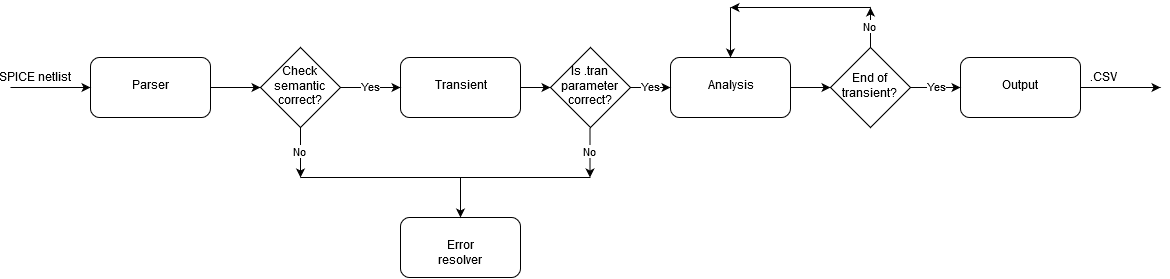
\includegraphics[width = \textwidth]{Program flow}
        \caption{Program flowchart}
        \label{fig:Netlist input example}
    \end{figure}
    \subsection{Git management}
    The feature each teammate is responsible for will be implemented in a feature branch until it is fully tested and
    other teammates are familiarised with its interface. \par
    Xin Wang will be in charge of Git repo management responsibilities.
    \subsection{Milestones}
    \begin{itemize}
        \item v1.0: 
        \begin{itemize}
            \item Basic nodal analysis possible with resistor and independent sources.
            \item \textbf{Transient not possible yet, only calculates one instance in time.}
        \end{itemize}  
        \item v2.0: 
        \begin{itemize}
            \item Transient analysis ability implemented.
            \item Dependent sources supported.
        \end{itemize}
        \item v3.0:
        \begin{itemize}
            \item Capacitor and Inductor supported.
        \end{itemize}
        \item Codebase optimisation.
        \item v4.0:
        \begin{itemize}
            \item Non-linear components supported.
        \end{itemize}
        \item Codebase optimisation.
    \end{itemize}

\end{document}    
